\documentclass[conference]{IEEEtran}
\IEEEoverridecommandlockouts

\usepackage[T1]{fontenc}
\usepackage{cite}
\usepackage{amsmath,amssymb}
\usepackage{booktabs}
\usepackage{graphicx}
\usepackage{url}
\usepackage{xcolor}
\usepackage{tikz}
\usetikzlibrary{positioning,arrows.meta,fit,calc,backgrounds}
\usepackage{pgfplots}
\pgfplotsset{compat=1.18}

\makeatletter
\newcommand{\tabinput}[1]{\@@input #1 }
\makeatother

\newcommand{\rev}{\operatorname{Rev}}
\newcommand{\EQ}{\textsc{eq}}
\newcommand{\FE}{\textsc{fe}}
\newcommand{\BE}{\textsc{be}}
\newcommand{\NEG}{\textsc{neg}}
\newcommand{\trackhead}{%
  & \multicolumn{3}{c}{T1 EN} & \multicolumn{3}{c}{T2 ES} & \multicolumn{3}{c}{T3 EU}
  & \multicolumn{3}{c}{T4 Mixed} & \multicolumn{3}{c}{ALL-4} \\
  \cmidrule(lr){2-4}\cmidrule(lr){5-7}\cmidrule(lr){8-10}\cmidrule(lr){11-13}\cmidrule(lr){14-16}
  System & F1 & S & H & F1 & S & H & F1 & S & H & F1 & S & H & F1 & S & H \\}

\definecolor{enc}{HTML}{DCE8F5}
\definecolor{dec}{HTML}{FBE8D3}
\definecolor{io}{HTML}{EFEFEF}
\definecolor{prior}{HTML}{E4F2E1}
\tikzset{
  box/.style={draw, rounded corners=2pt, align=center, font=\footnotesize,
              inner sep=3pt, minimum height=7mm},
  arr/.style={-{Stealth[length=2mm]}, semithick},
}

\begin{document}

\title{Consistency by Construction: Cross-Encoders with Reversal-Aware Decoding
for SemEval-2027 Task~2 (DiCo-NLI)}

\author{\IEEEauthorblockN{Le Duc Minh}}

\maketitle

\begin{abstract}
DiCo-NLI asks a system to label an ordered phrase pair as equivalence, forward
entailment, backward entailment or another relation, and then checks whether
the labels it gives to $(a,b)$ and $(b,a)$ agree. We fine-tune multilingual
cross-encoders and move consistency out of training and into decoding: the
log-probabilities of a pair and its reversed twin are mapped into one frame,
averaged, and decoded once, so every pair predicted as reversible is
consistent by construction. On the development set, a seven-model ensemble
reaches a Weighted F1 of 80.8, SoftCons of 95.7 and HardCons of 88.0,
averaged over the English, Spanish, Basque and mixed tracks. Almost all
remaining errors separate the negative class from the three entailment
labels. Five methods aimed at that decision, including focal loss, extra iSTS
data and a stacked classifier, did not beat the plain ensemble. If the
reversible/negative split is read from the layout of the input files, scores
rise to 92.6, 100 and 91.2, above the current development leader. We report
that variant separately because it depends on how the data were packaged.
\end{abstract}

\begin{IEEEkeywords}
natural language inference, directional consistency, cross-encoders,
multilingual NLP, Basque, SemEval
\end{IEEEkeywords}

\section{Introduction}

Natural language inference (NLI) models are usually scored one example at a
time. A model can do well on that score and still contradict itself, for
example by labelling both $(a,b)$ and $(b,a)$ as forward entailment, which
would make each phrase strictly more specific than the other. SemEval-2027 Task~2, DiCo-NLI~\cite{dicoNLIsite,dicoNLIrepo}, makes
this visible. Every reversible phrase pair appears in both orders, and systems
are scored on per-example Weighted F1 and on two consistency measures over the
pairs.

Our system is built around one observation: consistency can be enforced at
decoding time for free, because both directions of every reversible pair are
in the same input file. We average the two directions' scores in a shared
frame and choose a single label for the pair. This leaves the classifier with
one job, which is to separate the entailment family from everything else.
That job turned out to be the hard part. The contributions of this report are
the decoding scheme and an exactly reversal-equivariant variant of the
cross-encoder, a comparison of four multilingual backbones, and a negative
result: none of the five \NEG-focused methods we tried improved on a plain
ensemble. Code, configurations and run logs are
public.\footnote{\url{https://github.com/MinLee0210/dico-nli-challenge}}

\section{Task and Data}

Each instance is an ordered pair $(a,b)$ of short phrases, about six words in
total, taken from the chunk alignments of PhrasIS~\cite{phrasis2024}, which in
turn come from the interpretable STS datasets of SemEval
2015--2016~\cite{semeval2015sts,semeval2016ists,lopezgazpio2017ists}. The label
is \EQ, \FE{} ($a \models b$), \BE{} ($b \models a$) or \NEG, where \NEG{}
covers every other PhrasIS relation (similar, related, opposite). The reversal
map is $\rev(\EQ)=\EQ$, $\rev(\FE)=\BE$ and $\rev(\BE)=\FE$; \NEG{} has no
reverse. There are four tracks: English (T1), Spanish (T2), Basque (T3) and
mixed-language pairs (T4).

Weighted F1 is the support-weighted F1 over the four labels. SoftCons counts
a gold-reversible pair as consistent when both predictions are reversible and
$\rev$-compatible, whatever the gold label. HardCons requires both directions
to be correct. Predicting \NEG{} on either side of a gold-reversible pair
therefore costs both consistency scores at once, which makes a false \NEG{}
the most expensive error.

We checked three facts on every training and development file. Instance ids
have the form \texttt{<pair\_id>\_\_<l1>-<l2>\_\_<original|flipped>}, and the
reversed twin swaps both the language codes and the direction tag. Every
reversible instance has its twin in the same file, while every \NEG{} instance
appears once. A \texttt{pair\_id} is shared across tracks, with two rows in
each monolingual track and twelve in T4. Each monolingual track has 3{,}042
training rows (1{,}282 reversible pairs and 478 \NEG) and 660 development rows
(277 and 106).

\section{Related Work}

Interpretable STS~\cite{lopezgazpio2017ists,semeval2016ists} introduced the
chunk-level relation types from which PhrasIS and DiCo-NLI are derived.
Consistency of neural models under logical transformations has been studied
for NLI~\cite{minervini2018adversarially,li2019logic} and for question
answering~\cite{ribeiro2019red}, usually through extra loss terms. For
symmetric pair tasks, Xu et al.~\cite{xu2019symmetric} and Kumar and
Joshi~\cite{kumar2022striking} penalise disagreement between the two input
orders; we use the same idea for an antisymmetric label set, where the two
orders should agree up to the $\rev$ map. Our \NEG{} study draws on work
showing that NLI models lean on lexical overlap~\cite{hans2019} and fail on
simple lexical inferences~\cite{glockner2018breaking}, and on focal
loss~\cite{lin2017focal} and intermediate-task transfer~\cite{pruksachatkun2020intermediate}
as remedies. For Basque we rely on multilingual encoders; XLM-R-large was the
strongest of the multilingual encoders evaluated on XNLIeu~\cite{xnlieu2024};
Basque-specific language models such as Latxa~\cite{latxa2024} are larger
decoders that we did not try.

\section{System}

\subsection{Cross-encoder}
A pretrained encoder reads \texttt{[CLS]}~$a$~\texttt{[SEP]}~$b$~\texttt{[SEP]}
and a linear head maps the first-token state to four
logits~\cite{bert2019,wolf2020transformers}. We use
DeBERTa-v3~\cite{deberta2021,debertav3} for English only, and three
multilingual backbones: mmBERT-base~\cite{mmbert2025}, an mDeBERTa-v3-base
checkpoint fine-tuned on multilingual NLI data~\cite{laurer2023universal,laurer2024less},
and XLM-R-large~\cite{xlmr2020} fine-tuned on XNLI~\cite{xnli2018,multinli2018}.
Multilingual models are trained on all four tracks at once (27{,}378 rows),
so each source pair is seen in nine language combinations.

\subsection{Consistency-aware decoding}
Fig.~\ref{fig:overview} shows the decoding pipeline. For an instance $x$ with
log-probabilities $\ell(x)\in\mathbb{R}^4$, the canonical score is
$\tilde\ell(x)=\ell(x)$ for \texttt{original} rows and $\tilde\ell(x)=P\,\ell(x)$
for \texttt{flipped} rows, where the permutation $P$ swaps the \FE{} and \BE{}
coordinates. Instances are grouped and the mean of $\tilde\ell$ over a group
is decoded to one canonical label, after adding a bias $\beta$ to the \NEG{}
score:
\begin{equation}
  y^\ast = \arg\max_{c}\; \Bigl(\tfrac{1}{|G|}\textstyle\sum_{x\in G}\tilde\ell_c(x)
  + \beta\,[c=\NEG]\Bigr).
\end{equation}
Original rows receive $y^\ast$ and flipped rows receive $\rev(y^\ast)$. With
\emph{independent} grouping each instance is its own group, which is plain
argmax. \emph{Twin} grouping joins an instance with its reversed twin.
\emph{Source} grouping joins every row with the same \texttt{pair\_id} in the
decoded file, which pools language views in T4. Any group holding both
directions is $\rev$-consistent by construction. All per-track results in this
report decode each track file on its own.

\begin{figure*}[t]
\centering
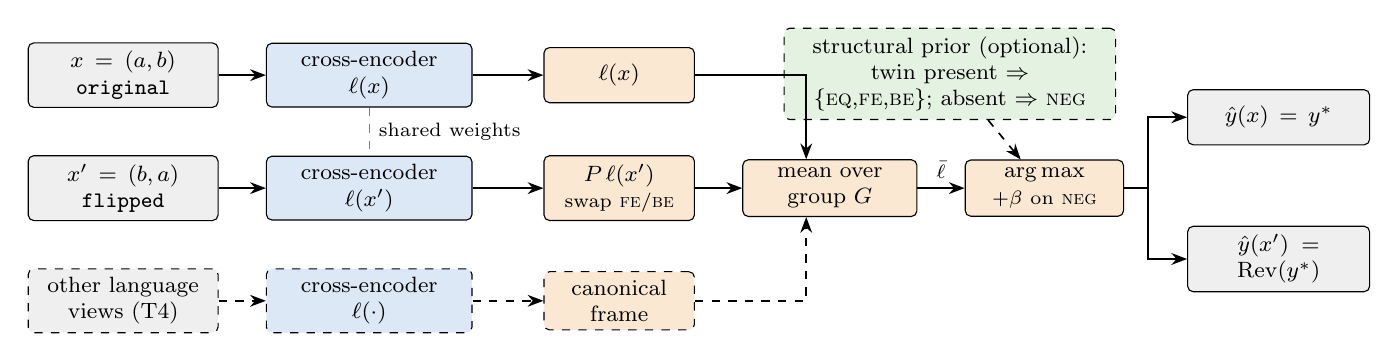
\begin{tikzpicture}[node distance=5mm and 6mm]
  % inputs
  \node[box, fill=io, text width=22mm] (x1) {$x=(a,b)$\\\texttt{original}};
  \node[box, fill=io, text width=22mm, below=6mm of x1] (x2) {$x'=(b,a)$\\\texttt{flipped}};
  \node[box, fill=io, text width=22mm, below=6mm of x2, dashed] (x3) {other language\\views (T4)};
  % encoder
  \node[box, fill=enc, text width=24mm, right=of x1] (e1) {cross-encoder\\$\ell(x)$};
  \node[box, fill=enc, text width=24mm, right=of x2] (e2) {cross-encoder\\$\ell(x')$};
  \node[box, fill=enc, text width=24mm, right=of x3, dashed] (e3) {cross-encoder\\$\ell(\cdot)$};
  \draw[dashed, gray] (e1) -- node[right, font=\scriptsize, text=black] {shared weights} (e2);
  % canonical frame
  \node[box, fill=dec, text width=17mm, right=9mm of e1] (c1) {$\ell(x)$};
  \node[box, fill=dec, text width=17mm, right=9mm of e2] (c2) {$P\,\ell(x')$\\{\scriptsize swap \FE/\BE}};
  \node[box, fill=dec, text width=17mm, right=9mm of e3, dashed] (c3) {canonical\\frame};
  % pooling
  \node[box, fill=dec, text width=20mm, right=of c2] (pool) {mean over\\group $G$};
  \node[box, fill=dec, text width=18mm, right=of pool] (arg) {$\arg\max$\\{\scriptsize $+\beta$ on \NEG}};
  % outputs
  \node[box, fill=io, text width=21mm, right=8mm of arg, yshift=9mm] (o1) {$\hat y(x)=y^\ast$};
  \node[box, fill=io, text width=21mm, right=8mm of arg, yshift=-9mm] (o2) {$\hat y(x')=\rev(y^\ast)$};
  % structural prior
  \node[box, fill=prior, dashed, text width=40mm, above=5mm of arg, xshift=-12mm] (sp)
    {structural prior (optional):\\twin present $\Rightarrow$ \{\EQ,\FE,\BE\}; absent $\Rightarrow$ \NEG};
  % arrows
  \draw[arr] (x1) -- (e1); \draw[arr] (x2) -- (e2); \draw[arr, dashed] (x3) -- (e3);
  \draw[arr] (e1) -- (c1); \draw[arr] (e2) -- (c2); \draw[arr, dashed] (e3) -- (c3);
  \draw[arr] (c1.east) -| ($(pool.north)+(-3mm,0)$);
  \draw[arr] (c2) -- (pool);
  \draw[arr, dashed] (c3.east) -| ($(pool.south)+(-3mm,0)$);
  \draw[arr] (pool) -- node[above, font=\scriptsize] {$\bar\ell$} (arg);
  \draw[arr] (arg.east) -- ++(3mm,0) |- (o1);
  \draw[arr] (arg.east) -- ++(3mm,0) |- (o2);
  \draw[arr, dashed] (sp) -- (arg);
\end{tikzpicture}
\caption{Consistency-aware decoding. Scores of an instance and its reversed
twin (and, in T4, of other language views of the same source pair) are mapped
into the \texttt{original} frame, averaged, and decoded once. The reversed row
receives the reversed label, so the pair is consistent whenever it is not
\NEG. The optional structural prior restricts the choice using the file layout.}
\label{fig:overview}
\end{figure*}

\subsection{Symmetric architecture}
Decoding gives consistency only when both directions are in the input. We
also built a model that is consistent for any single input. It scores both
orders with the same encoder $f$ and combines them as
\begin{equation}
  g(a,b) = \tfrac12\bigl(f(a,b) + P\,f(b,a)\bigr),
\end{equation}
so $g(b,a)=P\,g(a,b)$ holds exactly (Fig.~\ref{fig:symmetric}). The cost is
two forward passes per example. A unit test checks the identity to within
$10^{-5}$.

\begin{figure}[t]
\centering
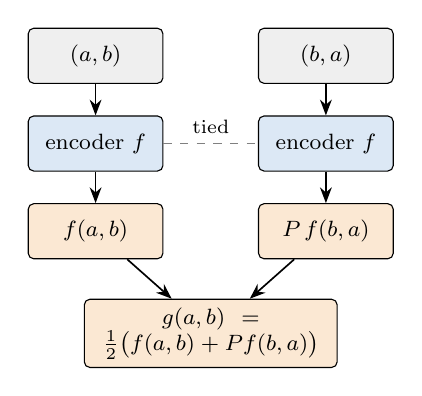
\begin{tikzpicture}[node distance=4mm and 5mm]
  \node[box, fill=io, text width=15mm] (ab) {$(a,b)$};
  \node[box, fill=io, text width=15mm, right=12mm of ab] (ba) {$(b,a)$};
  \node[box, fill=enc, text width=15mm, below=of ab] (f1) {encoder $f$};
  \node[box, fill=enc, text width=15mm, below=of ba] (f2) {encoder $f$};
  \draw[dashed, gray] (f1) -- node[above, font=\scriptsize, text=black] {tied} (f2);
  \node[box, fill=dec, text width=15mm, below=of f1] (l1) {$f(a,b)$};
  \node[box, fill=dec, text width=15mm, below=of f2] (l2) {$P\,f(b,a)$};
  \node[box, fill=dec, text width=30mm, below=5mm of $(l1.south)!0.5!(l2.south)$] (avg)
    {$g(a,b)=\tfrac12\bigl(f(a,b)+P f(b,a)\bigr)$};
  \draw[arr] (ab) -- (f1); \draw[arr] (ba) -- (f2);
  \draw[arr] (f1) -- (l1); \draw[arr] (f2) -- (l2);
  \draw[arr] (l1) -- (avg); \draw[arr] (l2) -- (avg);
\end{tikzpicture}
\caption{The symmetric model scores both input orders with one encoder and
averages the results after swapping \FE{} and \BE{} on the reversed side.
Swapping $a$ and $b$ therefore swaps \FE{} and \BE{} in the output exactly.}
\label{fig:symmetric}
\end{figure}

\subsection{Training objectives}
The loss is cross-entropy, optionally with label smoothing~\cite{szegedy2016rethinking},
plus a reversal-consistency term between each row and its twin, which a
twin-aware batch sampler keeps in the same batch:
\begin{equation}
  \mathcal{L} = \mathrm{CE} + \lambda\,\mathrm{KL}_{\mathrm{sym}}\bigl(p(x)\,\|\,P\,p(x')\bigr).
\end{equation}
For the \NEG{} study we added class-weighted and focal~\cite{lin2017focal}
variants of the cross-entropy term and a \emph{reverse-negative} augmentation
that adds the reversed copy of each \NEG{} pair; \NEG{} is its own reverse, so
the label stays correct.

\subsection{Structural prior}
The second data fact makes the reversible-or-\NEG{} decision readable from the
file: a group whose reversed twin is present is decoded among \EQ, \FE{} and
\BE, and a group without a twin is decoded as \NEG. This is exact on training
and development data. It is a property of how the files were built, not of
the phrases, and the test files may be packaged differently, so we report
every result with and without it. \emph{Prior-aware} models are trained on the
three reversible labels only, since under the prior the model is never asked
about \NEG; they must not be used without it.

\section{Experimental Setup}

All models were trained on one NVIDIA RTX~4000~Ada (20\,GB) with mixed
precision, AdamW~\cite{loshchilov2019decoupled}, 10\% linear warm-up and linear
decay, batch size 16--32 and maximum length 64--128 subword tokens. Learning
rates were $2\cdot10^{-5}$ for DeBERTa-v3-base, $5\cdot10^{-5}$ for mmBERT,
$1.5\cdot10^{-5}$ for mDeBERTa and $10^{-5}$ for XLM-R-large. The symmetric
XLM-R model used batch size 8 to fit in memory. The multilingual models reach
their best score within the first epoch, so for the main runs we validate
every 15\% of an epoch and stop after five checks without improvement.

The early-stopping monitor is the mean of the three official scores with the
four development files decoded together. It is only used to stop training and
to compare runs quickly; every table decodes each track separately. Ensembles
average log-probabilities before decoding~\cite{lakshminarayanan2017deep}.
Our metric code agrees with the official scorer to machine precision on all
tracks and decoding modes, and the headline results were re-scored with the
official scorer.

\section{Results}

\subsection{Decoding}
Table~\ref{tab:decoding} isolates decoding on a single DeBERTa-v3-base model
for T1. Twin decoding costs 0.6 F1 points and gains 5.4 SoftCons and 2.5
HardCons points. SoftCons stays below 100 only because some reversible pairs
are predicted as \NEG. With the structural prior, the same model scores
exactly what the development leader reports for T1 (92.4 / 100 / 91.0), which
suggests the leader uses the same prior.

\begin{table}[t]
\centering
\caption{Decoding modes for one DeBERTa-v3-base model on the T1 development
set. Best value per column in bold.}
\label{tab:decoding}
\begin{tabular}{lccc}
\toprule
Decoding & W-F1 & SoftCons & HardCons \\
\midrule
independent & 82.7 & 88.1 & 83.8 \\
twin        & 82.1 & 93.5 & 86.3 \\
source      & 82.1 & 93.5 & 86.3 \\
twin + structural prior & \textbf{92.4} & \textbf{100.0} & \textbf{91.0} \\
\bottomrule
\end{tabular}
\end{table}

\begin{table}[!t]
\centering
\caption{Methods aimed at the negative class: ALL-4 development scores
without the prior. Best value per column in bold.}
\label{tab:neg}
\begin{tabular}{lccc}
\toprule
System & W-F1 & SoftCons & HardCons \\
\midrule
A (mDeBERTa)            & 79.4 & 95.9 & 87.0 \\
\quad + \NEG{} weight 2  & 79.7 & 91.2 & 83.1 \\
\quad + focal, $\gamma=2$ & 78.2 & 94.4 & 85.9 \\
\quad + reverse negatives & 80.2 & 91.2 & 83.1 \\
\quad + iSTS answers-students & 77.8 & 96.2 & 87.0 \\
\midrule
B (XLM-R-large)         & 78.8 & 96.3 & 86.3 \\
\quad + reverse negatives & 74.3 & 92.7 & 79.6 \\
\quad + iSTS answers-students & 77.6 & 92.8 & 84.3 \\
\midrule
Clean-7 ensemble        & 80.8 & 95.7 & 88.0 \\
\quad + stacked \NEG{} detector & \textbf{81.4} & 91.8 & 84.7 \\
\quad with $\beta=-1.0$ & 79.1 & \textbf{98.5} & \textbf{89.8} \\
\bottomrule
\end{tabular}
\end{table}

\begin{figure}[!t]
\centering
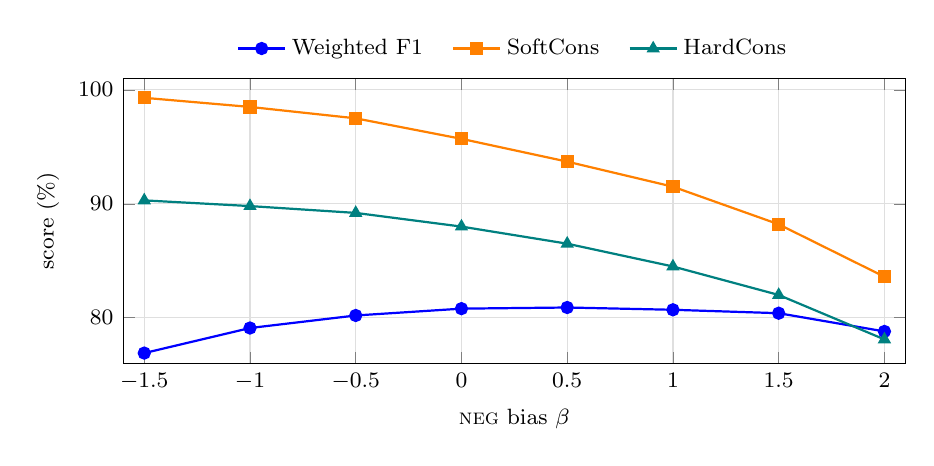
\begin{tikzpicture}
\begin{axis}[
  width=0.95\columnwidth, height=5.2cm,
  xlabel={\NEG{} bias $\beta$}, ylabel={score (\%)},
  xmin=-1.6, xmax=2.1, ymin=76, ymax=101,
  xtick={-1.5,-1,-0.5,0,0.5,1,1.5,2},
  legend style={font=\footnotesize, at={(0.5,1.03)}, anchor=south, draw=none, legend columns=3,
                /tikz/every even column/.append style={column sep=3mm}},
  tick label style={font=\footnotesize}, label style={font=\footnotesize},
  grid=major, grid style={gray!25},
]
\addplot[thick, blue, mark=*] coordinates
  {(-1.5,76.9) (-1,79.1) (-0.5,80.2) (0,80.8) (0.5,80.9) (1,80.7) (1.5,80.4) (2,78.8)};
\addplot[thick, orange, mark=square*] coordinates
  {(-1.5,99.3) (-1,98.5) (-0.5,97.5) (0,95.7) (0.5,93.7) (1,91.5) (1.5,88.2) (2,83.6)};
\addplot[thick, teal, mark=triangle*] coordinates
  {(-1.5,90.3) (-1,89.8) (-0.5,89.2) (0,88.0) (0.5,86.5) (1,84.5) (1.5,82.0) (2,78.1)};
\legend{Weighted F1, SoftCons, HardCons}
\end{axis}
\end{tikzpicture}
\caption{Effect of the \NEG{} bias $\beta$ on the clean seven-model ensemble
(ALL-4 development scores). Lowering $\beta$ trades F1 for consistency.}
\label{fig:bias}
\end{figure}

\subsection{Backbones and model variants}
Tables~\ref{tab:clean} and~\ref{tab:prior} give per-track development scores
without and with the structural prior. The two NLI-trained encoders,
mDeBERTa and XLM-R-large, are close to each other and well ahead of mmBERT,
which starts from masked-language-model weights and overfits after one epoch.
A Basque-only encoder trained on T3 alone (JaunBERT) reached a monitor score
of only 76.9, so we kept the multilingual models for Basque. The symmetric
architecture does not help a single model, and adding it to the clean
ensemble lowers HardCons from 88.0 to 87.3. With consistency already enforced
at decoding time, the architectural guarantee adds nothing here.

On T1, the English-only DeBERTa-v3-large reaches 83.3 / 95.3 / 88.1, but the
multilingual ensemble already scores 83.7 / 95.3 / 89.9 and adding the large
model does not change it. Seed and backbone ensembles give the only
consistent gains. The best clean system averages seven models (four mDeBERTa
and three XLM-R-large seeds) and reaches 80.8 / 95.7 / 88.0 over the four
tracks.

With the prior, the prior-aware models are the strongest single models, and
the best system averages fourteen of them. It reaches 92.6 / 100 / 91.2 over
the four tracks, above the development leader (91.4 / 100 / 89.7) on T1, T3,
T4 and the average, and slightly below it on T2.

\begin{table*}[t]
\centering
\caption{Development results without the structural prior (F1 = Weighted F1,
S = SoftCons, H = HardCons, in \%). A = mDeBERTa, fine-grained validation;
B = XLM-R-large XNLI. Single seeds except ensembles. Best value per column in
bold.}
\label{tab:clean}
\resizebox{\textwidth}{!}{%
\begin{tabular}{l*{15}{c}}
\toprule
\trackhead
\midrule
\tabinput{tables/dev_clean.tex}
\bottomrule
\end{tabular}}
\end{table*}

\begin{table*}[t]
\centering
\caption{Development results with the structural prior, and the CodaBench
development leader on 29 September 2026. Best value per column among our
systems in bold; columns where all systems tie are not marked.}
\label{tab:prior}
\resizebox{\textwidth}{!}{%
\begin{tabular}{l*{15}{c}}
\toprule
\trackhead
\midrule
\tabinput{tables/dev_prior.tex}
\midrule
Leaderboard \#1 & 92.4 & 100 & 91.0 & 92.8 & 100 & 91.3 & 90.3 & 100 & 88.4 & 90.2 & 100 & 88.2 & 91.4 & 100 & 89.7 \\
\bottomrule
\end{tabular}}
\end{table*}

\subsection{The negative class}
Without the prior, the three reversible labels are rarely confused with each
other; the errors that remain are almost all \NEG{} against the rest. We tested
five ways to improve that decision (Table~\ref{tab:neg}).

Class weighting (weight 2 on \NEG) and focal loss ($\gamma=2$) lowered HardCons
on mDeBERTa by 3.9 and 1.1 points. Reverse-negative augmentation gained 0.8 F1
points on mDeBERTa but cost 4.7 SoftCons points, and hurt XLM-R-large on every
metric. We then added 1{,}010 chunk pairs from the iSTS 2016
answers-students data, mapping EQUI to \EQ, SPE1 and SPE2 to \FE{} and \BE, and
SIMI, REL and OPPO to \NEG. We did not use the headlines and images subsets,
because they are the source of PhrasIS and contain its test pairs, and none of
the converted pairs occurs in the DiCo training or development data. The extra
data lowered F1 for both backbones, and a second mDeBERTa seed was also
worse.

The last method was a stacked detector. A logistic regression and a
gradient-boosted classifier predict \NEG{} from the single-row log-probabilities
of the seven ensemble members and from lexical features (token overlap,
containment, length, number mismatch, negation words), with five-fold
cross-validation grouped by \texttt{pair\_id}. The best setting raised F1 by
0.6 points but lowered SoftCons by 3.9 and HardCons by 3.3. The ensemble's own
\NEG{} score seems to carry the same lexical signal already.

Moving the \NEG{} threshold $\beta$ only trades one score for another
(Fig.~\ref{fig:bias}). Lowering it towards $-1.5$ lifts HardCons to 90.3 and
SoftCons to 99.3 while F1 falls to 76.9; raising it does the reverse. The mean
of the three scores stays between 88 and 89 over the whole range.



\subsection{Cross-track pooling}
Because a \texttt{pair\_id} is shared by all tracks, decoding the four
development files together pools up to eighteen views of each source pair. In
a four-model ensemble with the prior this added about one point of both F1
and HardCons over per-track decoding (92.7 / 100 / 91.3 against
91.8 / 100 / 90.3). It also uses the other tracks' inputs to predict a
given track and makes the four tracks' predictions identical, so we leave it
out of the reported results until the organizers say whether it is allowed.

\section{Discussion}

Two caveats apply to every number above. First, all model, ensemble and
threshold choices were made on the development set, which has 277 reversible
pairs per track; the standard error of HardCons at that size is about 2.6
points, so differences of one or two points between single runs are within
noise, and the reported scores are optimistic. Grouped cross-validation over
the training and development data would give firmer estimates. Second, the
lead over the leaderboard depends entirely on the structural prior. Without
it, our best system is about eleven points of F1 behind, and the gap is the
\NEG{} decision.

The negative results are consistent with what is known about NLI models on
short, lexically overlapping inputs~\cite{hans2019,glockner2018breaking}: the
hard \NEG{} cases are phrases that are related, similar or opposite, and more
weight, more data of the same kind or extra surface features did not teach the
models to separate them. Methods that change the model's inductive bias rather
than its training signal, such as larger instruction-tuned models used as
teachers, are the obvious next step.

\section{Conclusion}

Consistency in DiCo-NLI can be guaranteed by decoding the two directions of a
pair together, which raises SoftCons and HardCons at no training cost. With
that in place, the task reduces to deciding whether a phrase pair stands in an
entailment relation at all. Our clean seven-model ensemble reaches 80.8 / 95.7
/ 88.0 on the development set; the same models with a layout-based prior reach
92.6 / 100 / 91.2. Whether that prior may be used in the evaluation phase is a
question for the organizers.

\bibliographystyle{IEEEtran}
\bibliography{refs}

\end{document}
